\documentclass[12pt,a4paper]{article}
\usepackage[utf8]{inputenc}
\usepackage[russian]{babel}
\usepackage[left=2.00cm, right=2.00cm, top=2.00cm, bottom=2.00cm]{geometry}
\linespread{1.25}
\usepackage{setspace}
\usepackage{indentfirst}
\setlength{\parindent}{1.25cm}
\let\paragraph\ignorespaces
\usepackage{tabularx}
\usepackage{multirow}
\usepackage{graphicx}



\begin{document}
	
\begin{titlepage}
	
\begin{center}
	\large Университет ИТМО\\[5cm]
	\LARGE Практическая работа №4\\
	\normalsize по дисциплине <<Визуализация и моделирование>>\\[5cm]
\end{center}
\begin{flushright}
		\begin{minipage}{0.6\textwidth}
		\begin{flushleft}
			\large
			\singlespacing 
			\textbf{Автор:} Костылев Иван Михайлович\\
			\textbf{Поток:} 1.1\\
			\textbf{Группа:} K3240\\
			\textbf{Факультет:} ИКТ\\
			\textbf{Преподаватель:} Чернышева А.В.
		\end{flushleft}
	\end{minipage}
\end{flushright}

\vfill

\begin{center}
	{\large Санкт-Петербург, \the\year{ г.}}
\end{center}
 
\end{titlepage}
\normalsize


\large \textbf{Описание датасета}

\normalsize
	Датасет состоит из данных о студентах, их родителей и оценок, полученных ими по различным предметам. \\

Всего записей: 1000 \\


\large \textbf{Формальное описание}

\begin{tabular}{ | p{100pt} | p{100pt} | p{100pt} | p{40pt} | p{60pt} |}
\hline
Столбец & Описание & Значения & Формат & Шкала  \\ \hline
gender & пол студента & male / female & текст & Качеств номинальная \\ \hline
race/ethnicity & расовая классификация & group A / group B / group C / group D & текст & Качеств номинальная  \\ \hline
parental level of education & уровень образования родителей & collegue / school / bachelor's degree / others  & текст & Качеств номинальная  \\ \hline
lunch & оплата обеда & standart / free/reduced & текст & Качеств номинальная  \\ \hline
test preparation & подготовка к тесту & none / completed & текст & Качеств номинальная  \\ \hline
math score & оценка по математике & 0..100 & целое число & Колич относительная  \\ \hline
reading score & оценка по чтению & 0..100 & целое число & Колич относительная  \\ \hline
writting score & оценка по письму & 0..100 & целое число & Колич относительная  \\ \hline
\end{tabular}
\\
\\

\textbf{Предобработка данных}
\\ 
Подобранный датасет не нуждался в предобработке на устранение пустых ячеек. Категориальные данные будем приводить из строк к числовому типу по мере необходимости.

\newpage

\textbf{Описательная статистика 2.0} \\

Здесь можно лишь показать, что данные являются цельными, без пустых ячеек.

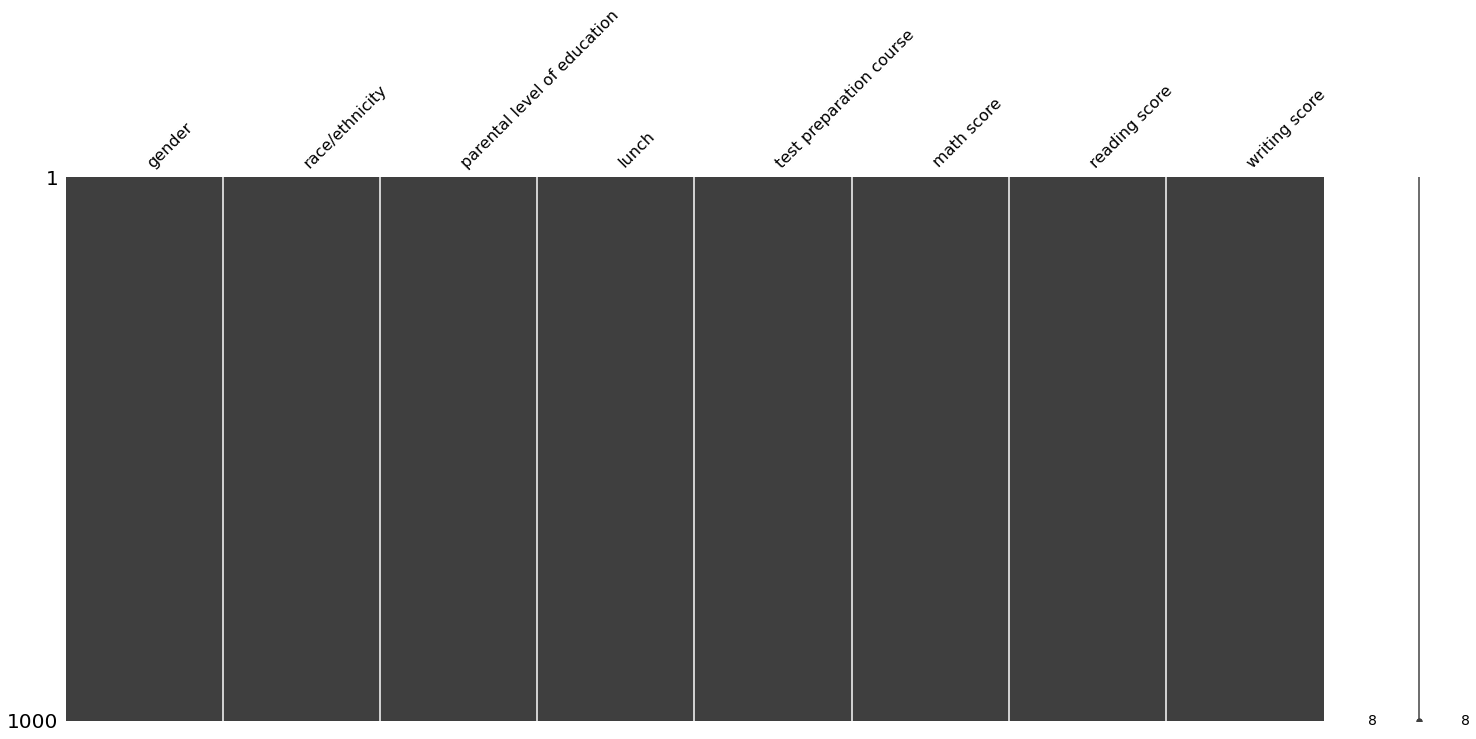
\includegraphics[scale=0.3]{msno_matrix} \\

С предыдущего этапа не произошло никаких качественных изменений в данных, которые могли бы позволить получить какое-то новое понимание о данных, поэтому проводить описательную статистику снова не имеет смысла. \\

\textbf{Новые гипотезы}\\


\textbf{1. Гипотеза: распределение оценок по предметам соответствует нормальному распределению} \\

\begin{verbatim}
sns.displot(df, x=READING, kde=True)
sns.displot(df, x=WRITING, kde=True)
sns.displot(df, x=MATH, kde=True)
\end{verbatim} 


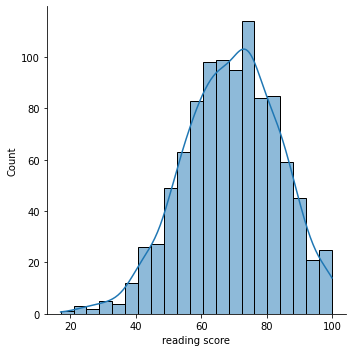
\includegraphics{scores_reading} \\
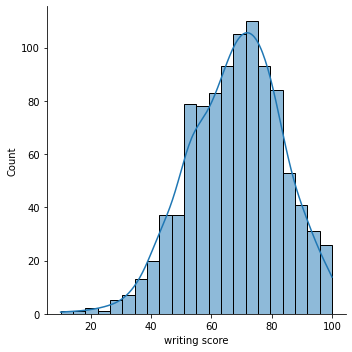
\includegraphics{scores_writing} \\
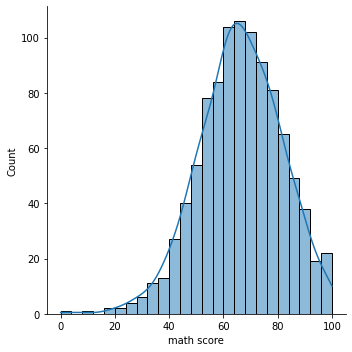
\includegraphics{scores_math} \\

\textbf{Вывод:} распределение оценок действительно является похожим на  нормальное. Теперь хотелось бы посмотреть более детально на данный график, как хорошо справлялись мужчины и женщины.


\textit{Из предыдущих исследований было видно, что женщины, в среднем, лучше справляются с работами (суммарный балл выше в среднем, чем у мужчин).} \\

\textbf{2. Вопрос: каково распределение баллов по предметам? Везде ли лидируют женщины?} \\

Построим аналогичный график, который будет отдельно показывать количество текущего балла у мужчин и женщин.\\


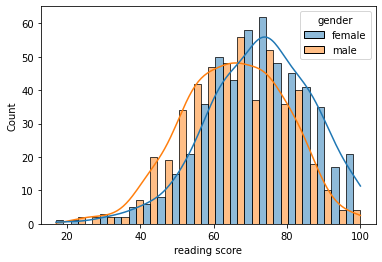
\includegraphics{scores_mf_reading} \\

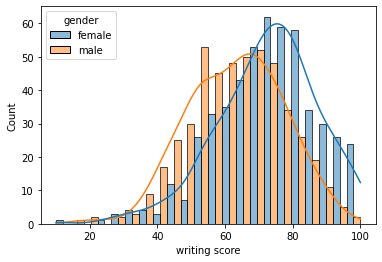
\includegraphics{scores_mf_writing} \\

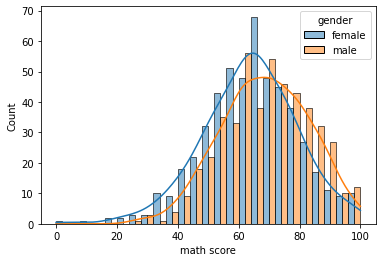
\includegraphics{scores_mf_math} \\

Здесь оранжевый график показывает распределение баллов у мужчин. Видно, что максимум правее у мужчин только в математике, т.е. можно утверждать, что мужчины справляются лучше только с математикой. Причем в этом предмете отрыв не такой большой, как в письме и чтении у женщин от мужчин. \\

\textit{Давайте построим большую матрицу корреляции, к которой сделаем несколько гипотез и вопросов.
}\\


\textbf{3. Удостоверимся, что оценки по чтению и письму коррелируют с полом студента (поскольку там явно выражено преобладание студентов-женщин по оценкам)}\\

\textbf{4. Гипотеза: Данные по уровню образования родителей коррелируются с наличием подготовки студентов к тесту. Студенты, родители которых имеют высшее образование, проходят подготовительные курсы, поскольку являются более ответственными.}\\

\textbf{5. Гипотеза: Уровень образования родителей коррелирует с расовой принадлежностью}\\


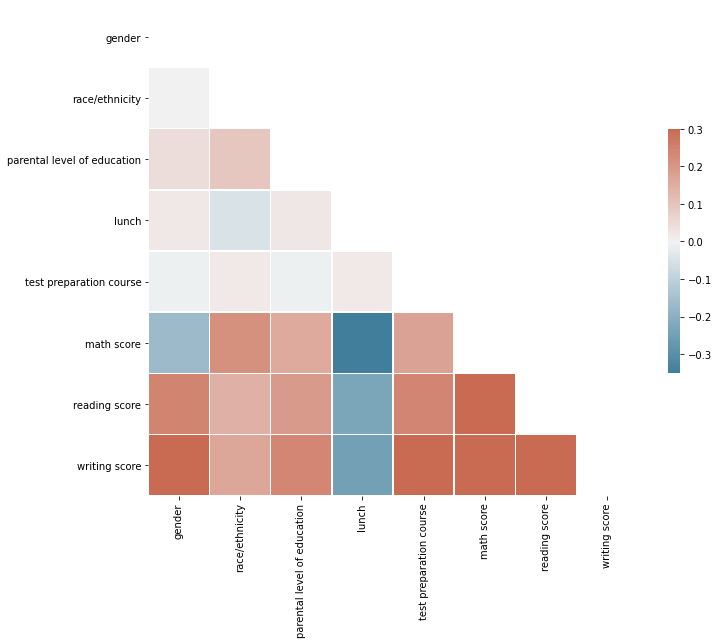
\includegraphics[scale=0.6]{matrix_corr} \\

3. Оценки по чтению больше всего коррелируют с гендером по письму и чтению - гипотеза подтвердилась. По математике корреляция меньше, поскольку мужчины чуть лучше справлялись с предметами, тогда как по письму и чтению виделось явное преобладание баллов у женщин.\\

4. Удивительно, но уровень образования родителей не делает студентов "более ответственными" и не гарантирует, что они будут проходить подготовительные курсы. В то же время уровень образования родителей коррелирует с оценками по предметам достаточно хорошо.\\

5. На данной матрице видно, что уровень образования родителей в общем и целом каким-то образом соответствует расовой принадлежности.\\

\textbf{Общие выводы по работе:} на основе проведенного исследования мы получили новую информацию о взаимосвязи между данными, что позволит строить более конкретные гипотезы в будущем и ставить какие-либо задачи.\\

К вопросам и задачам на будущее я бы отнес:\\
1) Как именно связана расовая принадлежность и уровень образования (какая этническая группа имеет более высокий уровень образования?)\\

2) Как именно связаны оценки по предметам с расой / уровнем образования родителей? \\

3) Каким образом можно смотреть на поле lunch? Видно, что есть небольшая корреляция с подготовительным курсом и с уровнем образования родителей. \\

\end{document}